\documentclass[10pt,a4paper]{article}
\usepackage[utf8]{inputenc}
\usepackage{amsmath}
\usepackage{amsfonts}
\usepackage{amssymb}
\usepackage{booktabs}
\usepackage{tikz}
\usepackage{adjustbox}
\usepackage{caption}  
\usepackage{multirow}
\usepackage{algorithm}
\usepackage[noend]{algpseudocode}
\usepackage{listings}
\usepackage{xcolor}
\usepackage{pgfopts}
\usepackage{xstring}


\usetikzlibrary{positioning,angles,quotes,calc,shapes.geometric}
\usetikzlibrary{chains,shapes.multipart}
\usetikzlibrary{shapes,calc,fit}
\usetikzlibrary{automata,positioning}


\lstset{
language=Java,
basicstyle=\small\ttfamily,			
keywordstyle=\color{blue},
commentstyle=\color{gray},			
stringstyle=\color{black},			
numbers=left,						
numberstyle=\tiny,					
stepnumber=1,						
breaklines=true						
}


\begin{document}



\section{Goal}




\section{Conceptual Model}

Let's start with the \textit{second} step of a typical discrete-event simulation: the \textbf{conceptual model} building. 

First of all our system represents a network of nodes to which some application, running in set of external mobile devices, send their tasks, called \textbf{jobs}, because of performance or energy saving reasons. 

Not all job sent to system are the same, in fact we make distinction between two types of task, denoted as \textbf{class 1 job} and \textbf{class two job}; differences betweens them are described in following sections. 

To minimize mean response time experienced by mobile device users, the system is been built as a "\textit{two-layer}" network in such a way that an arriving job is sent, if possible, firstly to the nearest node.

\begin{adjustbox}{center=\textwidth}
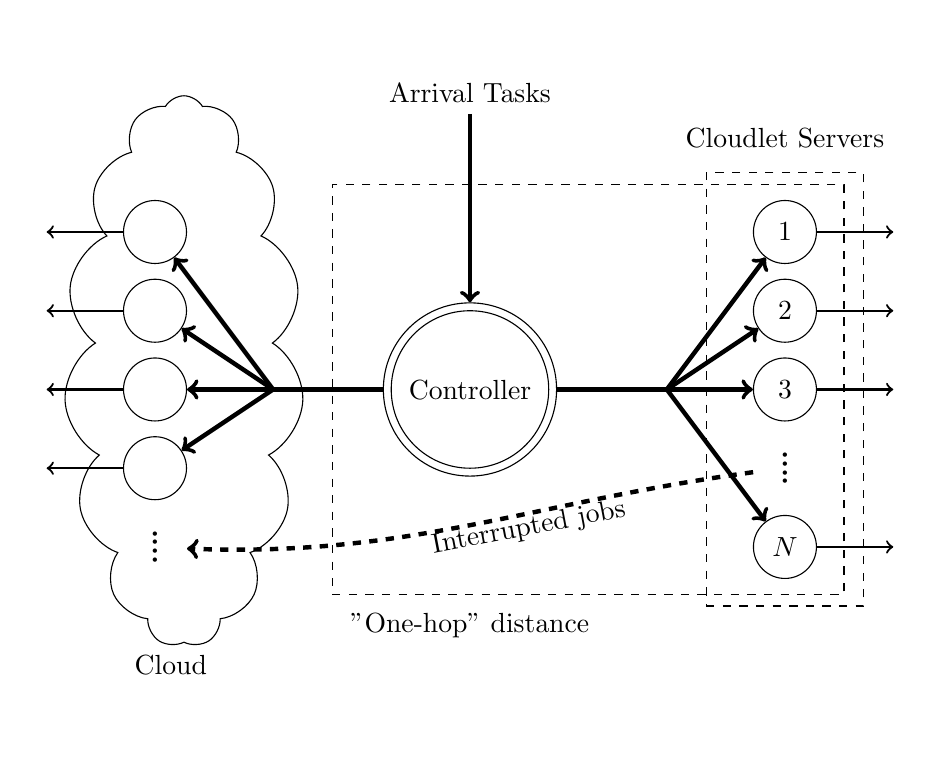
\begin{tikzpicture}


% Cloud

\node[circle, draw, minimum width = 0.8cm]        					   (CloudNode0) at (0,2) {};
\node[circle, draw, minimum width = 0.8cm, below of=CloudNode0]        (CloudNode1) {};
\node[circle, draw, minimum width = 0.8cm, below of=CloudNode1]        (CloudNode2) {};
\node[circle, draw, minimum width = 0.8cm, below of=CloudNode2]        (CloudNode3) {};
\node[circle, draw=white, minimum width = 0.8cm, below of=CloudNode3]  (CloudNode4) {\rotatebox{90}{\textbf{....}}};

\node[above of=CloudNode4, yshift=-2.5cm, xshift=0.2cm] (labellllllll) {Cloud};

\node[right of=CloudNode0, xshift=-2.5cm] (ExtCloudNode0) {};
\node[right of=CloudNode1, xshift=-2.5cm] (ExtCloudNode1) {};
\node[right of=CloudNode2, xshift=-2.5cm] (ExtCloudNode2) {};
\node[right of=CloudNode3, xshift=-2.5cm] (ExtCloudNode3) {};


\coordinate (cloudStartNode) at (1.5,0);

% Controller

\node[circle, draw, minimum width = 2.2cm]  (ControllerExternal) at (4,0) {};
\node[circle, draw, minimum width = 2cm]    (Controller2)        at (4,0) {Controller};

\coordinate (cloudletStartNode) at (6.5,0);

\coordinate (Start) at (4,3.5);

% Cloudlet

\node[circle, draw, minimum width = 0.8cm, left of=ControllerExternal, xshift=5cm, yshift=2cm]       (CloudletNode0) {$1$};
\node[circle, draw, minimum width = 0.8cm, below of=CloudletNode0]           (CloudletNode1) {$2$};
\node[circle, draw, minimum width = 0.8cm, below of=CloudletNode1]           (CloudletNode2) {$3$};
\node[circle, draw=white, minimum width = 0.8cm, below of=CloudletNode2]     (CloudletNode3) {\rotatebox{90}{\textbf{....}}};
\node[circle, draw, minimum width = 0.8cm, below of=CloudletNode3] (CloudletNode4) {$N$};

\node[rectangle, draw, dashed, minimum width =6.5cm, minimum height=5.2cm] (Cloudlet) at (5.5,0) {};
\node[circle,below of=Cloudlet, yshift=-2cm, xshift=-1.5cm] (label1) {"One-hop" distance};

\node[left of=CloudletNode0, xshift=2.5cm] (ExtCloudletNode0) {};
\node[left of=CloudletNode1, xshift=2.5cm] (ExtCloudletNode1) {};
\node[left of=CloudletNode2, xshift=2.5cm] (ExtCloudletNode2) {};
\node[left of=CloudletNode4, xshift=2.5cm] (ExtCloudletNode3) {};

\node[rectangle, draw, dashed, minimum width =2cm, minimum height=5.5cm, right of=CloudletNode2, xshift=-1cm] (CloudletFrame) {};
\node[circle,above of=CloudletFrame, yshift=2.2cm] (label1) {Cloudlet Servers};

% Cloudlet Rows...

\draw[ultra thick,-] (ControllerExternal) -- (cloudletStartNode);
\draw[ultra thick,->] (cloudletStartNode) -- (CloudletNode0);
\draw[ultra thick,->] (cloudletStartNode) -- (CloudletNode1);
\draw[ultra thick,->] (cloudletStartNode) -- (CloudletNode2);
\draw[ultra thick,->] (cloudletStartNode) -- (CloudletNode4);

% Cloud Rows...

\draw[ultra thick,-] (ControllerExternal) -- (cloudStartNode);
\draw[ultra thick,->] (cloudStartNode) -- (CloudNode0);
\draw[ultra thick,->] (cloudStartNode) -- (CloudNode1);
\draw[ultra thick,->] (cloudStartNode) -- (CloudNode2);
\draw[ultra thick,->] (cloudStartNode) -- (CloudNode3);

% Out from cloudlet nodes

\draw[thick,->] (CloudletNode0) -- (ExtCloudletNode0);
\draw[thick,->] (CloudletNode1) -- (ExtCloudletNode1);
\draw[thick,->] (CloudletNode2) -- (ExtCloudletNode2);
\draw[thick,->] (CloudletNode4) -- (ExtCloudletNode3);

% Out from cloud nodes

\draw[thick,->] (CloudNode0) -- (ExtCloudNode0);
\draw[thick,->] (CloudNode1) -- (ExtCloudNode1);
\draw[thick,->] (CloudNode2) -- (ExtCloudNode2);
\draw[thick,->] (CloudNode3) -- (ExtCloudNode3);
 
% START

\draw[ultra thick,->] (Start) node[above] {Arrival Tasks} -- (ControllerExternal) ;

\node [cloud, right of=CloudNode3, xshift=-18, yshift=35, draw,cloud puffs=15,cloud puff arc=120, aspect=3, minimum width =2.5cm, minimum height=7cm, inner ysep=1em] (cloudcc) {};

\path (CloudletNode3) edge[->,dashed,ultra thick, bend left, out=0, in=170] node [left] [sloped, yshift=-5,xshift=60] {Interrupted jobs} (CloudNode4);

\end{tikzpicture}
\end{adjustbox}



To be more precise, our system is made up of a set of nodes described below:

\begin{description}
\item[Cloudlet] It represents an \textit{edge cloud server} which, in addition to being located at "\textit{one-hop}" distance from mobile devices users, and therefore nearest to them, is able to guarantee absence of interferences among tasks allocated to it as long as their number does not exceed a given threshold $N$. From our conceptual model point of view, cloudlet represents a \textbf{fixed-capacity multi-server service node with any queue}.

Its capacity, that is the maximum possible number of jobs in it, is fixed to $N$

\item[Cloud] It represents a \textit{remote cloud server} which, although it \textbf{suffers for greater network delay}, due of its high distance from mobile devices, has virtually \textbf{unlimited resources} so that he can to process any number of tasks allocated to it. Consequently we had modelled this subsystem as an \textbf{unlimited-capacity multi-server service node with any queue}.

Being made up of an unlimited number of servers, its capacity is also unlimited.

\item[Controller] It represent the entry point of our system because all task are sent to it from outside in order to decide about whether an arrived job should be sent to the cloudlet or the cloud according to a given access control algorithm.

It is located on cloudlet and has the capability to precess each arriving job \textbf{instantaneously}. So that it is modelled simply as \textbf{single-server service node with no queue}. 

\end{description}

\begin{algorithm}

\caption{}\label{alg:accessControlAlgorithm1}

\begin{algorithmic}[1]

\Function{accessControlFunction}{$\textit{arrivalJob}$}

\If {$(n_1 + n_2=N)$}
	\State Send $\textit{arrivalJob}$ on the cloud.
\Else 	
 	\State Send $\textit{arrivalJob}$ on the cloudlet.
\EndIf

\EndFunction

\end{algorithmic}
\end{algorithm}

At this point, in order to properly define our conceptual model, we need to specify \textit{state variables} of our system. 
Due to access control algorithms characteristics, described below, we have decided to represent the state of our system as an ordered pair $(n_1, n_2)$ where $n_1$ represents the number of class one job while $n_2$ the number of class two job both contained in cloudlet. Consequently we have decided to just ignore type and number of jobs contained in cloud node because not relevant in any access control algorithms and negligible for goal of our study. 

A this point we can observe access control algorithms used by controller to make decisions which are fully described by their pseudo-code shown in Algorithm \ref{alg:accessControlAlgorithm1} and Algorithm \ref{alg:accessControlAlgorithm2}. 

Observe that to make its decision controller node can use only one access control algorithm at a time. 

Note that Algorithm \ref{alg:accessControlAlgorithm2} use a further threshold variable to make its decision denoted by $S$ which is less or equal than $N$. Remember that when a class 2 job is interrupted and sent on the cloud, a \textbf{ setup time} has to be considered to restart the task on the cloud. 

\begin{algorithm}
\caption{}\label{alg:accessControlAlgorithm2}
\begin{algorithmic}[1]

\Function{accessControlFunction}{$\textit{arrivalJob}$}

\If {$(\textit{arrivalJob.isClassOne})$}


\If {$n_1 = N$}
	\State Send $\textit{arrivalJob}$ on the cloud.

\ElsIf{$n_1 + n_2 \leq S $}
	\State Send $\textit{arrivalJob}$ on the cloudlet.
\ElsIf{$ n_2 \geq 0 $}
	\State Interrupt a class 2 job currently running on cloudlet.
	\State Send interrupted job to cloud.
	\State Send $\textit{arrivalJob}$ on the cloudlet.
\Else 	
 	\State Send $\textit{arrivalJob}$ on the cloudlet.
\EndIf



\Else 

\If {$(n_1 + n_2 \geq S)$}
	\State Send $\textit{arrivalJob}$ on the cloud.
\Else 	
 	\State Send $\textit{arrivalJob}$ on the cloudlet.
\EndIf

\EndIf

\EndFunction

\end{algorithmic}
\end{algorithm}

















\newpage
\section{Specification  Model}

In this section we will provide a \textit{specification model} of our system in which, as we know, system's states exist as a collection of mathematical variables together with equations and logic describing how the state variables are interrelated and an algorithm for computing their interaction and evolution in time\footnote{See. 186}.

\subsection{State variables}

In previous section we have said that system state is represented by the number, type, response of job running on each system's node. Now we will formalize 

\begin{table}[h!]
    \caption{System state variables.}
    \centering
    \small
    \label{table:StateVariables}
     \begin{tabular}{rcl}

      \toprule
      
      $n_{\text{global}}^{(1)}(t)$ & $ = $ & Class 1 job number currently running on overall system at time $t$ \\\\
	  $n_{\text{global}}^{(2)}(t)$ & $ = $ & Class 2 job number currently running on overall system at time $t$ \\\\
      
      $n_{\text{cloudlet}}^{(1)}(t)$ & $ = $ & Class 1 job number currently running on cloudlet at time $t$ \\\\
	  $n_{\text{cloudlet}}^{(2)}(t)$ & $ = $ & Class 2 job number currently running on cloudlet at time $t$ \\\\
         
      $n_{\text{cloud}}^{(1)}(t)$ & $ = $ & Class 1 job number currently running on cloud at time $t$ \\\\
	  $n_{\text{cloud}}^{(2)}(t)$ & $ = $ & Class 2 job number currently running on cloud at time $t$ \\\\
	  
	  $d_{\text{global}}^{(1)}(t)$ & $ = $ & Number of departed class 1 job on overall system at time $t$ \\\\
	  $d_{\text{global}}^{(2)}(t)$ & $ = $ & Number of departed class 1 job on overall system at time $t$ \\\\
      
      $d_{\text{cloudlet}}^{(1)}(t)$ & $ = $ & Number of departed class 1 job on cloudlet at time $t$ \\\\
	  $d_{\text{cloudlet}}^{(2)}(t)$ & $ = $ & Number of departed class 1 job on cloudlet at time $t$ \\\\
	  
	  $d_{\text{cloud}}^{(1)}(t)$ & $ = $ & Number of departed class 1 job on cloud at time $t$ \\\\
	  $d_{\text{cloud}}^{(2)}(t)$ & $ = $ & Number of departed class 1 job on cloud at time $t$ \\\\
    
      \bottomrule


    \end{tabular}
\end{table}
\newpage
\subsection{Time averaged statistics}

Using state variables previously described, we can compute all system's statistics which we need in very simple ways.

From now we will denote with $\tau \in (t_0, t)$ an instant of our system simulation where $t_0$ and $t$ are respectively its \textit{start moment} and \textit{final moment}. We will also use $c \in \lbrace 1,2 \rbrace = C$  to denote the class to which a job belongs while $x \in \lbrace cloudlet,cloud \rbrace = X$ will be used to refer to a specific system's node.

$E[N_j](c)$, \textbf{average number of class $c$ jobs into $j$}, can be computed as follows: 

\begin{equation}
\begin{array} {lcr} 
\displaystyle E[N_x](c) = \dfrac{1}{t-t_0}\int_{t_0}^t n_x^{(c)}(\tau)d\tau & \qquad & \forall c \in C, \forall x \in X
\end{array}
\end{equation}

To obtain $E[N_x]$, time average number of jobs into $x$, and $E[N]$, time average number of jobs into overall system, we can proceed as shown below:

\begin{equation}
\begin{array} {lcr} 
E[N_x] = \sum_{c \in C} E[N_x](c) & \qquad & \forall x \in X
\end{array}
\end{equation}

\begin{equation}
E[N] = \sum_{x \in X} E[N_x]
\end{equation}


Let's look now to \textbf{average response time experienced by class $c$ jobs into a system node $j$} $E[T_j](c)$.
In order to compute this statistic, we had to observe that our system hasn't queues therefore $E[T_j](c)$ is simply equal to $E[S_j](c)$, that is \textbf{average service time experienced by class $c$ jobs into a system node $j$}. We just have to show how to compute $E[S_j](c)$:

\begin{equation}
E[S_j](c) = \sum_{i=1}^N s_{i}
\end{equation}




To compute mean response time experienced by jobs, we had to observe that our system there are no queues, therefore 


\subsection{Events}

Having to built next-event simulation model, let's look to all possible \textbf{events} which can occurs during our simulation. We recall that, by definition, \textbf{an event is an occurrence that may change the state of the system}, therefore our system's state variables can only when an event occurs\footnote{See. 187}. All event capable to alter system's state are reported below:


\begin{table}[h!]
    \caption{System's events}
    \centering
    \small
    \label{table:StateVariables}
     \begin{tabular}{c|c|r|r}

      \toprule
      \multirow{2}{*}{\textbf{Event name}} & \multirow{2}{*}{\textbf{Event's place}} & \textbf{State variables} & \textbf{State variables} \\
      & & \textbf{incremented by one} & \textbf{decremented by one} \\
      \midrule
      
      \multirow{3}{*}{Class 1 Job arrival} & Cloudlet & $n_{\text{cloudlet}}^{(1)}(t)$ & \\ \cline{2-4}
      & Cloud & $n_{\text{cloud}}^{(1)}(t)$ & \\ \cline{2-4}
      & Controller & $n_{\text{system}}^{(1)}(t)$ & \\
       
      \hline
       
      \multirow{3}{*}{Class 2 Job arrival} & Cloudlet & $n_{\text{cloudlet}}^{(2)}(t)$ & \\ \cline{2-4}
      & Cloud & $n_{\text{cloud}}^{(2)}(t)$ & \\ \cline{2-4}
      & Controller & $n_{\text{system}}^{(2)}(t)$ & \\
    
	  \hline 
      \vspace{0.1cm}
      \multirow{2}{*}{Class 1 Job departure} & Cloudlet &
      $d_{\text{cloudlet}}^{(1)}(t)$, $d_{\text{system}}^{(1)}(t)$ &
      $n_{\text{cloudlet}}^{(1)}(t)$, $n_{\text{system}}^{(1)}(t)$ \vspace{0.1cm} \\ \cline{2-4}
    
      & Cloud & 
      $d_{\text{cloud}}^{(1)}(t)$, $d_{\text{system}}^{(1)}(t)$ &
      $n_{\text{cloud}}^{(1)}(t)$, $n_{\text{system}}^{(1)}(t)$ .\\
        
      \bottomrule


    \end{tabular}
\end{table}


Finally, to complete to turn out our conceptual model into a proper specification model, we have to make additional assumptions reported below:

\begin{itemize}
\item Although initial state variables can have any non-negative integer value\footnote{See. pag 190}, we have choosen, as common, to set $n_x^{(j)}(0) = 0$ and $d_x^{(j)}(0) = 0$ setting, in this way, initial system status as \textbf{idle}. 

\item As a consequence of the previous point, first event must be either a \textbf{Class 1 Job arrival} or a
\textbf{Class 2 Job arrival} both on controller node.

\item Terminal state is also idle. Rather than specifying the number of jobs processed, our stopping criteria has been specified in terms of a time $\tau$ beyond which no new jobs can arrive. This assumption effectively closes the door at time $\tau$ but allows the system to continue operation until all jobs have been completely served. 

Therefore, the last event must be either a class 1 or class 2 job completion.
\end{itemize}


\newpage
\section{Computational Model}

Let's start now the description of \textit{computational model} in which system's states exist as a collection of data structure, classes and variables that collectively characterize the system and are systematically updated as simulated time evolves.

In order to build discrete-event simulation models using \textit{next-event} approach we need to:

\subsection{Events implementation}





In order to properly describe our computational model, we take a look how all system's events, seen in previous section, are implemented and managed.
First of all, a \textit{generic} event has been implemented and represented using an \textit{abstract} java class called \texttt{SimulationEvent} which has following features:

\begin{itemize}
\item Has only one \texttt{double} type field, used to hold instant of time according to which an event occurs.
\item Exports the signature of two very important abstract method, used by our simulation algorithm which we will describe next, called \texttt{perform()}, used to update system's state variables when an event occurs, and \texttt{scheduleFollowingEvent()}, which is used, instead, to inserts into an \textit{event list} the event that follows the current one.
\end{itemize}

As we said previously, these methods are abstract therefore their exact behaviour depends strictly by which class implements it. Is very important to specify that aforesaid class does \textit{not} represent events of our specific system but generic ones only. In order to represent a system-specific event, we have used another abstract class, a subclass of previous one, called \texttt{SystemEvent} which main feature is knowledge about \textit{event place}, that is in which system's component a specific event occurs. Concrete event classes that fully implements previously said abstract methods are listed below:

\begin{itemize}
\item \texttt{Class1JobArrival}
\item \texttt{Class2JobArrival}
\item \texttt{Class1JobDeparture}
\item \texttt{Class2JobDeparture}
\end{itemize}

These classes, having knowledge about which system's component is involved, can update state variable of that component and not of the others. For example a \textbf{Class2JobDeparture} event involving cloud node will update cloud state variables only. 

From software engineering point view, these concrete classes are unknown to the others, that is any class knows about their implementation; in fact, using factory method pattern for concrete class building and previously mentioned interfaces we can take advantage of polymorphism pattern to provide high cohesion and low coupling between our project classes.

\begin{lstlisting}[frame=lines, caption={Implementazione della funzione \texttt{start\_server}}, label={code:serverStart}]
public abstract class SystemEvent extends SimulationEvent {

    protected SystemComponent systemComponent;

    public void setSystemComponent(SystemComponent systemComponent) {
        this.systemComponent = systemComponent;
    }

    public SystemComponent getSystemComponent() {
        return systemComponent;
    }
    ...
\end{lstlisting}

\subsection{Event list}

As known, an \textit{event list}, also called \textit{calendar}, represents a data structure used to keep track of scheduled time of occurrence for the next possible event.
For reasons of efficiency, our event list is been implemented as a \textit{min-heap binary tree}, that is a \textit{priority queue} in which all possible event are ordered by time in such a way that the most imminent event is found on the tree's root, providing $O(log_2(n))$ time for the en-queuing and dequeuing operation and constant time for root element retrieval.\footnote{Camil Demetrescu, Irene Finocchi, Giuseppe F. Italiano - \textit{Algorimti e strutture dati} - second edition, McGraw-Hill, pag. 200} 

Luckily aforesaid data structure is already available in JDK through a very simple to use Java built-in class called \texttt{PriorityQueue$<$E$>$} which provides all method that we need although requires that all events object implement an interface called \texttt{Comparable} to work properly. Implementing that interface requires to define a method called \texttt{compareTo}, of which we have reported our implementation in listing \ref{code:compareTo}, in order to provide a total ordering among all possible event 
Observer that \texttt{compareTo} method returns a negative integer, zero, or a positive integer if an  this object is less than, equal to, or greater than the specified object.\footnote{See \texttt{https://docs.oracle.com/en/java/javase/12/docs/api/java.base/java/lang/Comparable.html\#compareTo(T)}}


\begin{lstlisting}[frame=lines, caption={Snippet of \texttt{SimulationEvent} class}, label={code:compareTo}]
@Override
public int compareTo(SimulationEvent o) {
	return Double.compare(this.startTime, o.startTime);
}
\end{lstlisting}




\subsection{Simulation clock}

As we know a simulated clock is necessary to keep track of the current value of simulated time during simulation. In our implementation this task is assigned to a class called 
\texttt{SimulationClock} which state is represented by a field holding current simulated time and another keeping instance of time according to which following event will occur.





\begin{lstlisting}[frame=lines, caption={Implementazione della funzione \texttt{start\_server}}, label={code:serverStart}]
public class SimulationClock {

    private static SimulationClock instance = null;

    private double currentEventTime;
    private double nextEventTime;

    private SimulationClock(){
    }

    public static SimulationClock getInstance() {
        if (instance == null)
            instance = new SimulationClock();
        return instance;
    }
    
    /* Getter and setter methods follow... */
\end{lstlisting}

The ways in which simulated clock is update is represented in listing; every 



\subsection{Next-event simulation logic}



\texttt{ComputationalModel} abstract class contains logic according to which a next next-event simulation is based on. That logic is written into \texttt{perform()} method, shown in listing \ref{code:perform}, which consists of the following steps:

\begin{description}
\item[Simulation initialization] Through a call to \texttt{initializeSimulation()} method, all system's state variables, including simulation clock, are initialized. During this phase time of occurrence of the first possible events is determined and scheduled, initializing thereby the event list.
From implementation point view, observe that said method make a set of call to some abstract method which signature is present in the same class, therefore a concrete class implementing these method is required.

\item[Process current event] Until event list is not empty (line 6), the most imminent possible event is extracted and removed from event list (line 8), the simulation clock is then advanced to this event's scheduled time of occurrence (line 12) and finally system state is updated (line 14). 

\item[Schedule following event] Until a fixed simulation time $\tau$ in not exceeded, a new event is generated by current event and consequently placed into event list. Subsequently simulation clock instance field, used to holding time of occurrence of next possible event, is updated in order to compute some system metrics.

\item[Statistic update] While simulation advance from one event time to the next, calling an abstract method called \texttt{updateStatistics()}, all system's statistic metrics are updated.

\item[Simulation result generation] When simulation stops, produced data are 

\end{description}


\begin{lstlisting}[frame=lines, caption={Snippet of \texttt{perform} method}, label={code:perform}]
...
public void perform() {

        initializeSimulation();

        while (!this.simulationEventList.isEmpty()) {

            SimulationEvent actualEvent = this.simulationEventList.poll();

            if (actualEvent != null) {

                SimulationClock.getInstance().setCurrentEventTime(actualEvent.getStartTime());

                actualEvent.perform();
                actualEvent.scheduleFollowingEvent();

                SimulationEvent nextEvent = this.simulationEventList.peek();

                if (nextEvent != null)
                    SimulationClock.getInstance().setNextEventTime(nextEvent.getStartTime());
            }
            updateStatistics();
        }

        produceStatisticResultsThroughBatchMeansMethod();

        printSimulationResults();
    }
...
\end{lstlisting}


\subsection{System implementation}

Let's try now to understand how our system implementatiuon is implemented.

Each node of our system is represented by an instance of SystemComponent class; 
SystemComponent is an abstract class that 

Our system's nodes are been implemented as a set of instance of some class that implements SystemComponent, which represent a generic system node. As shown from UML class diagram reported in /ref{fig:UMLSystemComponent}. 
That class provide methos used to update stare variable of a specified component invoked by SystemEvent objects when.


Each concrete class provide an implmentation 






\newpage
\section{Analytical solution}

In this last section we will develop an analytical solution to validate the results obtained previously through our simulations. 

\subsection{System based on access control Algorithm 1}
\begin{figure}
\caption{Access control algorithm 1 based cloudlet's CTMC.} \label{fig:ALG1-CloudletMarkovChain}
\begin{adjustbox}{center=\textwidth}
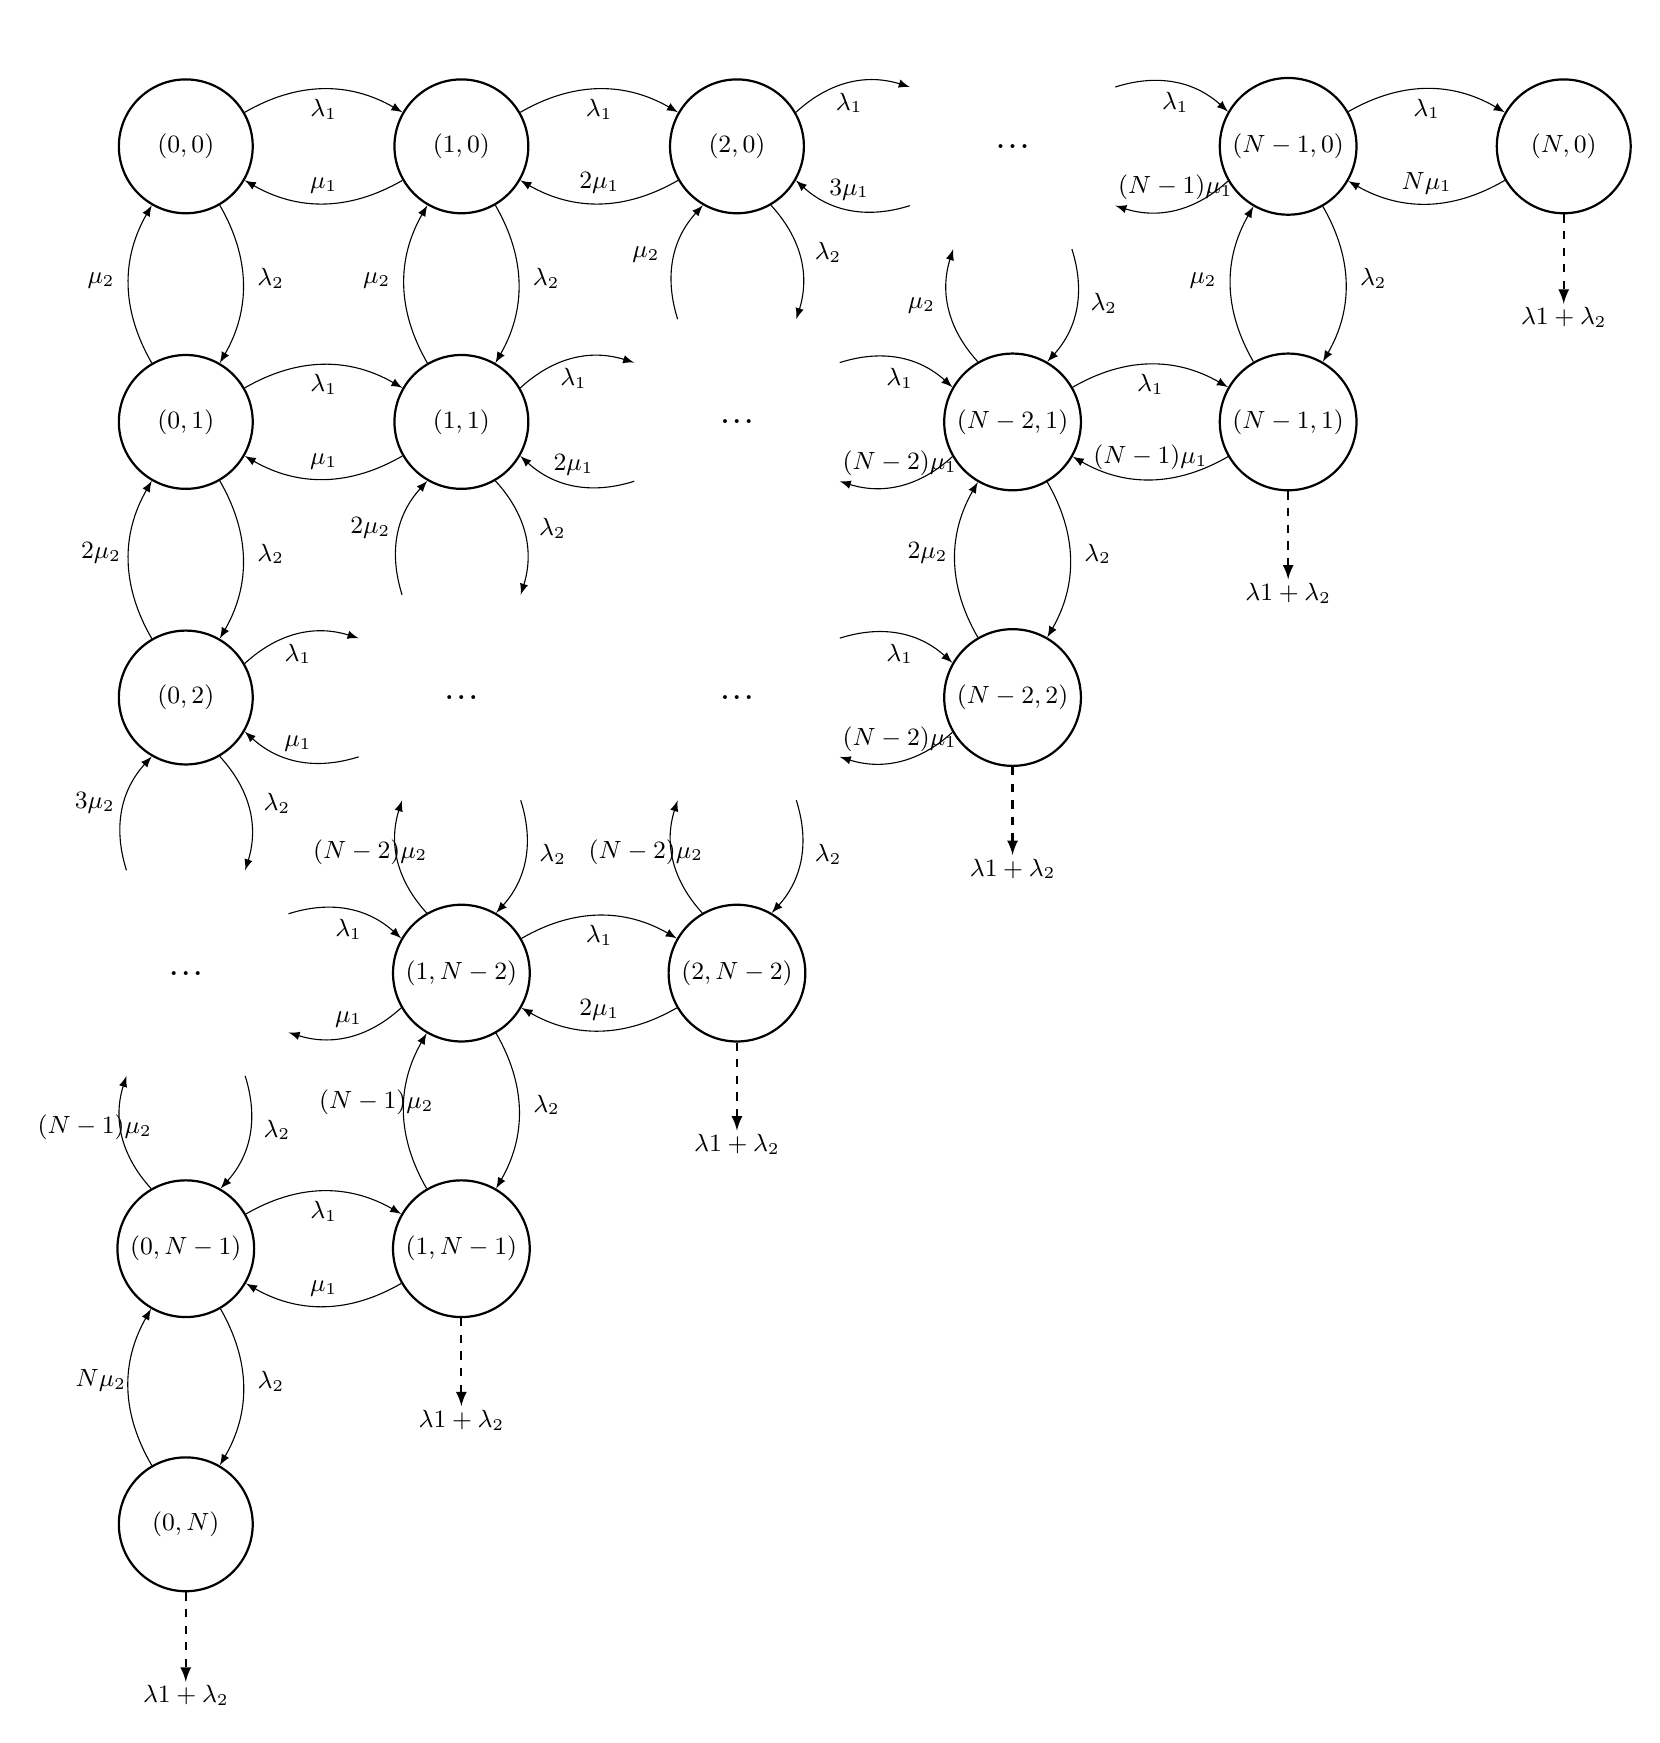
\begin{tikzpicture}[->,node distance=3.5cm,>=latex,font=\small, minimum width=1.7cm]

    \tikzstyle{round}=[thick,draw=black,circle]

    \node[round] 			    (00) {$(0,0)$};
    \node[round,right of=00]    (10) {$(1,0)$};
    \node[round,below of=00]    (01) {$(0,1)$};
    \node[round,below of=10]    (11) {$(1,1)$};
    \node[round,below of=01]    (02) {$(0,2)$};
    \node[round,right of=10]    (20) {$(2,0)$};
   
    \node[circle,draw=white,right of=20, minimum width = 3cm]    (A1) {\LARGE ...};
    \node[circle,draw=white,below of=02, minimum width = 3cm]    (A2) {\LARGE ...};
     
   	\node[round,right of=A1]    (N-1/0)  	{$(N-1,0)$};
   	\node[round,right of=N-1/0] (N0)	 	{$(N,0)$};
    \node[round,below of=N-1/0] (N-1/1)     {$(N-1,1)$};
    \node[round,left  of=N-1/1] (N-2/1)	{$(N-2,1)$};
    \node[round,below of=N-2/1] (N-2/2)	{$(N-2,2)$};
   
    \node[round,below of=A2]    (0/N-1)  	{$(0,N-1)$};
   	\node[round,below of=0/N-1] (0N)	 	{$(0,N)$};
    \node[round,right of=0/N-1] (1/N-1)     {$(1,N-1)$};
    \node[round,above of=1/N-1] (1/N-2)     {$(1,N-2)$};
    \node[round,right of=1/N-2] (2/N-2)	    {$(2,N-2)$};
    
    
    \node[circle,draw=white,left of=N-2/1,minimum width = 3cm]        (A3)     {\LARGE ...};
    \node[circle,draw=white,below of=11,minimum width = 3cm]          (A4)     {\LARGE ...};
    \node[circle,draw=white,above of=2/N-2,minimum width = 3cm]       (A5)     {\LARGE ...};
 
 	\draw[dashed,thick, ->] (N0) -- +(0,-2) node[yshift=-5]  {$\lambda1+\lambda_2$};
 	\draw[dashed,thick, ->] (N-1/1) -- +(0,-2) node[yshift=-5]  {$\lambda1+\lambda_2$};
 	\draw[dashed,thick, ->] (N-2/2) -- +(0,-2) node[yshift=-5]  {$\lambda1+\lambda_2$};
 	\draw[dashed,thick, ->] (2/N-2) -- +(0,-2) node[yshift=-5]  {$\lambda1+\lambda_2$};
 	\draw[dashed,thick, ->] (1/N-1) -- +(0,-2) node[yshift=-5]  {$\lambda1+\lambda_2$};
 	\draw[dashed,thick, ->] (0N) -- +(0,-2) node[yshift=-5]  {$\lambda1+\lambda_2$};
 
 	\path 
 	(00) 	edge[bend left,below]		node 					    {$\lambda_1$}		(10)
 		 	edge[bend left,above]       node [xshift=10,yshift=-5]  {$\lambda_2$} 		(01)
 	
 	(10) 	edge[bend left,above]       node 						{$\mu_1$} 			(00)
 		 	edge[bend left,below]		node 					    {$\lambda_1$}		(20)
 		 	edge[bend left,above]       node [xshift=10,yshift=-5]  {$\lambda_2$} 		(11)
 	
    (01) 	edge[bend left,above]       node [xshift=-10,yshift=-5] {$\mu_2$} 			(00)
   		 	edge[bend left,below]		node 					    {$\lambda_1$}		(11)
   	     	edge[bend left,above]       node [xshift=10,yshift=-5]  {$\lambda_2$} 		(02)
   
    (20) 	edge[bend left,above]       node 						{$2\mu_1$} 			(10)
    		edge[bend left,below]		node 					    {$\lambda_1$}		(A1)
    		edge[bend left,above]       node [xshift=10,yshift=-5]  {$\lambda_2$} 		(A3)
   		    
    (02) 	edge[bend left,above]       node [xshift=-10,yshift=-5] {$2\mu_2$} 			(01)
    		edge[bend left,above]       node [xshift=10,yshift=-5]  {$\lambda_2$} 		(A2)
    		edge[bend left,below]		node 					    {$\lambda_1$}		(A4)
   
    (11) 	edge[bend left,above]       node [xshift=-10,yshift=-5] {$\mu_2$} 			(10)
   		 	edge[bend left,above]       node 						{$\mu_1$} 			(01)
   		 	edge[bend left,below]		node 					    {$\lambda_1$}		(A3)
   		 	edge[bend left,above]       node [xshift=10,yshift=-5]  {$\lambda_2$} 		(A4)
   
   	(N0) 	edge[bend left,above]       node 						{$N\mu_1$} 			(N-1/0)
   
   	(N-1/0) edge[bend left,below]		node 					    {$\lambda_1$}		(N0)
   			edge[bend left,above]       node [xshift=10,yshift=-5]  {$\lambda_2$} 		(N-1/1)
   			edge[bend left,above]       node 						{$(N-1)\mu_1$} 			(A1)
   
    (N-1/1) edge[bend left,above]       node [xshift=-10,yshift=-5] {$\mu_2$} 			(N-1/0)
    		edge[bend left,above]       node 						{$(N-1)\mu_1$} 		(N-2/1)
    
    (N-2/1) edge[bend left,below]		node 					    {$\lambda_1$}		(N-1/1)
    		edge[bend left,above]       node [xshift=-10,yshift=-5] {$\mu_2$} 			(A1)
    		edge[bend left,above]       node 						{$(N-2)\mu_1$} 		(A3)
    		edge[bend left,above]       node [xshift=10,yshift=-5]  {$\lambda_2$} 		(N-2/2)
    		
    (N-2/2) edge[bend left,above]       node [xshift=-10,yshift=-5] {$2\mu_2$} 			(N-2/1)
    		edge[bend left,above]       node 						{$(N-2)\mu_1$} 		(A5)
    
    (0N) 	edge[bend left,above]       node [xshift=-10,yshift=-5]	{$N\mu_2$} 			(0/N-1)
   
   	(0/N-1) edge[bend left,below]		node 					    {$\lambda_1$}		(1/N-1)
   			edge[bend left,above]       node [xshift=10,yshift=-5]  {$\lambda_2$} 		(0N)
   			edge[bend left,above]       node [xshift=-10,yshift=-5]	{$(N-1)\mu_2$} 		(A2)
   
    (1/N-1) edge[bend left,above]       node 						{$\mu_1$}  			(0/N-1)
    	    edge[bend left,above]       node [xshift=-10,yshift=-5]	{$(N-1)\mu_2$} 		(1/N-2)
    
    (1/N-2) edge[bend left,above]       node 						{$\mu_1$}  			(A2)
    		edge[bend left,above]       node [xshift=10,yshift=-5]  {$\lambda_2$} 		(1/N-1)
    		edge[bend left,above]       node [xshift=-10,yshift=-5]	{$(N-2)\mu_2$} 		(A4)
    		edge[bend left,below]		node 					    {$\lambda_1$}		(2/N-2)
    		
    (2/N-2) edge[bend left,above]       node 						{$2\mu_1$}  		(1/N-2)
    		edge[bend left,above]       node [xshift=-10,yshift=-5]	{$(N-2)\mu_2$} 		(A5)
    
    (A1)    edge[bend left,above]       node 						{$3\mu_1$} 			(20)
    	    edge[bend left,below]		node 					    {$\lambda_1$}		(N-1/0)
    	    edge[bend left,above]       node [xshift=10,yshift=-5]  {$\lambda_2$} 		(N-2/1)
    	    
    (A2)	edge[bend left,above]       node [xshift=10,yshift=-5]  {$\lambda_2$} 		(0/N-1)
    		edge[bend left,above]       node [xshift=-10,yshift=-5]	{$3\mu_2$} 			(02)
    		edge[bend left,below]		node 					    {$\lambda_1$}		(1/N-2)
    		
    (A3)    edge[bend left,below]		node 					    {$\lambda_1$}		(N-2/1)
    		edge[bend left,above]       node [xshift=-10,yshift=-5]	{$\mu_2$} 			(20)
    		edge[bend left,above]       node 						{$2\mu_1$} 			(11)
    
    (A4)    edge[bend left,above]       node [xshift=-10,yshift=-5]	{$2\mu_2$} 			(11)
    		edge[bend left,above]       node 						{$\mu_1$} 			(02)
    		edge[bend left,above]       node [xshift=10,yshift=-5]  {$\lambda_2$} 		(1/N-2)
    		
    (A5)    edge[bend left,above]		node [xshift=10,yshift=-5]  {$\lambda_2$}		(2/N-2)
    		edge[bend left,below]		node 					    {$\lambda_1$}		(N-2/2);

\end{tikzpicture}
\end{adjustbox}
\end{figure}

Let's start with presentation of analytical solution of system based on access control algorithm 1.

In order to compute all parameters and metrics of interest associated with above-mentioned system, due to cloudlet's limited resources according to which it can accept jobs until their number does not exceed a given threshold $N$, is crucial compute first the \textbf{fraction of jobs that are forwarded to cloudlet and to cloud}; to do it, we must compute at first probability according to which the sum of job of each class in cloudlet system is equal to that threshold. 

To determine this probability, we had modelled cloudlet with a \textbf{continuous-time Markov chain} (\textbf{CTMC}), of which you can see a graphical representationin Figure \ref{fig:ALG1-CloudletMarkovChain}, where each chain's state, denoted with $(n_1,n_2)$, is represented by the number of class 1 job, $n_1$, and class 2 job, $n_2$, present in system at a certain moment.



\subsubsection{Balance equation computing} 

Obviously we can compute \textbf{limiting probabilities} $\pi_{(n_1,n_2)}$, namely the probability according to which the chain is in a certain state, say $j$, independently of the starting state, say $i$, via \textbf{balance} (or \textbf{stationary}) \textbf{equations}, in which we can equate the rate at which the system leaves state $j$ with the rate at which the system enters state $j$ \footnote{\textit{Cfr.} Mor Harchol-Balter - \textit{Performance Modeling and Design of Computer Systems} - Carnegie Mellon University, Pennsylvania, pag. 237}, \textbf{remembering that limiting probabilities sum to 1} (i.e., $\sum_{j=0}^\infty \pi_j = 1$).
These balance equations, shown in table \ref{table:ALG1-CloudletBalanceEquationList}, are been resolved using a very simple MATLAB script called \texttt{MATLAB\_ALG1\_CTMC\_ResolverScript.m} in which each equation, previously generated through a Java script\footnote{Cfr. \texttt{CTMCResolverScriptGenerator.java} and \texttt{ResolverUsingRoutingAlgorithm1.java} files.}, is been resolved using a MATLAB function called \texttt{solve(eqn,var)}.\footnote{\textit{Cfr.} \texttt{https://www.mathworks.com/help/symbolic/solve.html}}. 

\begin{table}[h!]
    \caption{Balance equations.}
    \centering
    \small
    \begin{adjustbox}{center=\textwidth}
    \label{table:ALG1-CloudletBalanceEquationList}
     \begin{tabular}{rcll}

      \toprule

      $(\lambda_1 + \lambda_2)\pi_{(0,0)}$ & $=$ & $\mu_1\pi_{(1,0)} + \mu_2\pi_{(0,1)}$ \\\\
       
      $(\lambda_1 + \lambda_2 + n_1\mu_1)\pi_{(n_1,0)} $ & $=$ & $ \lambda_1\pi_{(n_1-1,0)} + \mu_1(n_1+1)\pi_{(n_1+1,0)} + \mu_2\pi_{(n_1,1)}$ & $\forall n_1 \in \mathbb{N} \cap [1, N-1]$ \\\\
      
      $(\lambda_1 + \lambda_2 + n_2\mu_2)\pi_{(0,n_2)} $ & $=$ & $ \lambda_2\pi_{(0,n_2-1)} + \mu_1\pi_{(1,n_2)} + \mu_2(n_2+1)\pi_{(0,n_2+1)}$ & $ \forall n_2 \in \mathbb{N} \cap [1, N-1]$ \\\\
      
      $\mu_1N\pi_{(N,0)}$ & $=$ & $\lambda_1\pi_{(N-1,0)}$ \\\\
      
      $\mu_2N\pi_{(0,N)}$ & $=$ & $\lambda_2\pi_{(0,N-1)}$ \\\\
      
      $(n_1\mu_1 + n_2\mu_2)\pi_{(n_1,n_2)} $ & $=$ & $ \lambda_1\pi_{(n_1-1,n_2)} + \lambda_2\pi_{(n_1,n_2-1)}$ & $\forall n_1,n_2 \in \mathbb{N} \cap [1, N-1] \mid n_1 + n_2 = N $ \\\\
      
      $(\lambda_1 + \lambda_2 + n_1\mu_1 + n_2\mu_2)\pi_{(n_1,n_2)} $ & $=$ & $ \lambda_1\pi_{(n_1-1,n_2)} + \lambda_2\pi_{(n_1,n_2-1)} + \mu_1(n_1+1)\pi_{(n_1+1,n_2)} $ & $\forall n_1,n_2 \in \mathbb{N} \cap [1, N-1] \mid n_1 + n_2 < N$\\
      && $+\; \mu_2(n_2+1)\pi_{(n_1,n_2+1)}$ & \\
      
      \bottomrule

    \end{tabular}
    \end{adjustbox}
\end{table}



\newpage
\subsubsection{Probabilities computing}

Having found the stationary probabilities, we can now find \textbf{$\Pi_{\text{SendToCloud}}$}, that is the \textbf{probability that an arriving job on controller has to be forwarded to cloud}. Observe that the class to which an arrival job belongs to is not important because, according to access control Algorithm 1, \textbf{jobs of both classes have same probability to be sent to cloud}. To be more precise, \textbf{$\Pi_{\text{SendToCloud}}$} is the probability that an arrival job find that the number of jobs present in cloudlet has exceeded threshold $N$, which occurs when $n_1 + n_2 = N$. Formally:

\begin{equation}
\begin{array} {lcl} 
\Pi_{\text{SendToCloud}} & = & P\lbrace{\text{An arrival job on controller sees $N$ jobs in cloudlet}}\rbrace \\\\

& = & \text{Limiting probability that there are $N$ jobs in system} \\\\

& = & \displaystyle \sum_{\substack{n_1, n_2 \in \mathbb{N} \cap [0, N] \\ n1+n2=N}} \pi_{(n_1,n_2)} \\
\end{array}
\end{equation}

At this point we can easily compute \textbf{$\Pi_{\text{SendToCloudlet}}$}, which instead represents the \textbf{probability according to which an arriving job on controller has to be accepted on cloudlet} and it is same for both job classes too.

\begin{equation}
\begin{array} {lcl} 
\Pi_{\text{SendToCloudlet}} & = & P\lbrace{\text{An arrival job on controller sees less than $N$ jobs in cloudlet}}\rbrace \\\\
& = & 1 - P\lbrace{\text{An arrival job on controller sees $N$ jobs in cloudlet}}\rbrace \\\\

& = & 1 - \Pi_{\text{SendToCloud}} \\\\
\end{array}
\end{equation}

\subsubsection{Average arrival rates}

Is $\lambda_i(c)$ the \textbf{total arrival rate into a system's component $i$ of class $c$ job}. Applying previous results, using an appropriate equation\footnote{\textit{Cfr.} \textit{Ivi}, pag. 315, equation (18.1)}, we can now compute per-class average arrival rates as follow:

\begin{equation}
\begin{array} {rcl}

\lambda_{\text{cloud}}(1) & = & \lambda_1\cdot \Pi_{\text{SendToCloud}} \\
\lambda_{\text{cloud}}(2) & = & \lambda_2\cdot \Pi_{\text{SendToCloud}} \\
\lambda_{\text{cloudlet}}(1) & = & \lambda_1\cdot \Pi_{\text{SendToCloudlet}} \\
\lambda_{\text{cloudlet}}(2) & = & \lambda_2\cdot \Pi_{\text{SendToCloudlet}} \\\\
\end{array}
\end{equation}

Then we get $\lambda_i$, that is \textbf{total arrival rate to system's component $i$}, by summing the per-class rates as follows:

\begin{equation}
\begin{array} {rcl}

\lambda_{\text{cloud}} & = & \lambda_{\text{cloud}}(1) + \lambda_{\text{cloud}}(2) \\
\lambda_{\text{cloudlet}} & = & \lambda_{\text{cloudlet}}(1) + \lambda_{\text{cloudlet}}(2) \\
\end{array}
\end{equation}


\subsubsection{Average population}

Is $E[N_i](c)$ the \textbf{average number of class $c$ jobs into a component $i$}. 

We can use previously computed stationary probabilities to get average population for cloudlet; it's enough to sum each state's limiting probability multiplied by corresponding number of job as follows:

\begin{equation}
\begin{array} {rcl} 
E[N_{\text{cloudlet}}](1) & = & \displaystyle \sum_{ (n_1, n_2) \in M} n_1 \cdot \pi(n_1,n_2) \\\\

E[N_{\text{cloudlet}}](2) & = & \displaystyle \sum_{ (n_1, n_2) \in M} n_2 \cdot \pi(n_1,n_2) \\\\

E[N_{\text{cloudlet}}] & = & E[N_{\text{cloudlet}}](1) + E[N_{\text{cloudlet}}](2) \\\\

& = & \displaystyle \sum_{ (n_1, n_2) \in M} (n_1 + n_2) \cdot \pi(n_1,n_2) \\\\

\end{array}
\end{equation}

Since we have modelled cloud component as a $M/M/\infty$ system, in which there is no job's waiting time due to presence of an infinite number of servers, we can simply to apply \textbf{Little’s Law}\footnote{\textit{Cfr.} \textit{Ivi}, pag. 95, theorem (6.1)} in order to get cloud's average population as shown in Equation \ref{equation:ALG-1}.

\begin{equation}
\label{equation:ALG-1}
\begin{array} {rcl} 
E[N_{\text{cloud}}](1) & = & \lambda_{\text{cloud}}(1) \cdot E[T_{\text{cloud}}](1)  \\\\

& = & \lambda_{\text{cloud}}(1) \cdot (E[T_{Q_{\text{cloud}}}](1) + E[S_{\text{cloud}}](1))  \\\\

& = & \lambda_{\text{cloud}}(1) \cdot (\frac{1}{\mu_{\text{cloud}}(1)}) \\\\

& = & \dfrac{\lambda_{\text{cloud}}(1)}{\mu_{\text{cloud}}(1)} \\

\end{array}
\end{equation}

Similarly:
 
\begin{equation}
\begin{array} {rcl} 
E[N_{\text{cloud}}](2) & = & \dfrac{\lambda_{\text{cloud}}(2)}{\mu_{\text{cloud}}(2)}
\end{array}
\end{equation}

\begin{equation}
\begin{array} {rcl} 
E[N_{\text{cloud}}] & = & E[N_{\text{cloud}}](1) + E[N_{\text{cloud}}](2)
\end{array}
\end{equation}

Finally we can get global average job populations as follows:

\begin{equation}
\begin{array} {rcl} 

E[N](1) & = & E[N_{\text{cloudlet}}](1) + E[N_{\text{cloud}}](1) \\\\

E[N](2) & = & E[N_{\text{cloudlet}}](2) + E[N_{\text{cloud}}](2) \\\\

E[N] & = & E[N](1) + E[N](2) 

\end{array}
\end{equation}


\subsubsection{Average response time}

Is $E[T_i](c)$ the \textbf{mean response time experienced by a class $c$ jobs into a component $i$}. 

In order to properly compute said metric for each system's component observe that:
\begin{itemize}
\item Knowing per-class average job population and per-class mean arrival rates, we can easily compute $E[T_i](c)$ using Little’s Law.
\item Since our system haven't queues, because of there is no waiting time experienced by jobs, is true that $E[T_i](c)$ is also equal to $E[S_i](c)$, that is \textbf{mean service time experienced by a class $c$ jobs into a component $i$}, which is equal to $1/\mu_i(c)$, where $\mu_i(c)$ \textbf{means average service rate at which a class $c$ jobs into a component $i$ is served}.
\end{itemize}

Therefore we can get these metric as follows.

\begin{equation}
\begin{array} {rcl} 
E[T_{\text{cloudlet}}](1) & = & \dfrac{E[N_{\text{cloudlet}}](1)}{\lambda_{\text{cloudlet}}(1)} \\\\

& = & E[S_{\text{cloudlet}}](1) \\\\

& = & \dfrac{1}{\mu_{\text{cloudlet}}(1)} \\\\
\end{array}
\end{equation}

\begin{equation}
\begin{array} {rcl} 
E[T_{\text{cloudlet}}](2) & = & \dfrac{E[N_{\text{cloudlet}}](2)}{\lambda_{\text{cloudlet}}(1)} \\\\

& = & E[S_{\text{cloudlet}}](2) \\\\

& = & \dfrac{1}{\mu_{\text{cloudlet}}(2)} \\\\
\end{array}
\end{equation}

\begin{equation}
\begin{array} {rcl} 
E[T_{\text{cloud}}](1) & = & \dfrac{E[N_{\text{cloud}}](1)}{\lambda_{\text{cloud}}(1)} \\\\

& = & E[S_{\text{cloud}}](1) \\\\

& = & \dfrac{1}{\mu_{\text{cloud}}(1)} \\\\
\end{array}
\end{equation}

\begin{equation}
\begin{array} {rcl} 
E[T_{\text{cloud}}](2) & = & \dfrac{E[N_{\text{cloud}}](2)}{\lambda_{\text{cloud}}(2)} \\\\

& = & E[S_{\text{cloud}}](2) \\\\

& = & \dfrac{1}{\mu_{\text{cloud}}(2)} \\\\
\end{array}
\end{equation}

At this point we can get global per-class mean response times as follows:

\begin{equation}
\begin{array} {lcl} 
E[T](1) & = & E[T_{\text{cloudlet}}](1)\cdot P\lbrace\text{An arrival class 1 job is sent to cloudlet}\rbrace \\
\\
& & +\; E[T_{\text{cloud}}](1)\cdot P\lbrace\text{An arrival class 1 job is sent to cloud}\rbrace \\
\\
& = & E[T_{\text{cloudlet}}](1)\cdot \Pi_{\text{SendToCloudlet}} + E[T_{\text{cloud}}](1)\cdot \Pi_{\text{SendToCloud}} \\

\end{array}
\end{equation}

Similarly:

\begin{equation}
\begin{array} {lcl} 
E[T](2) & = & E[T_{\text{cloudlet}}](2)\cdot P\lbrace\text{An arrival class 2 job is sent to cloudlet}\rbrace \\
\\
& & +\; E[T_{\text{cloud}}](2)\cdot P\lbrace\text{An arrival class 2 job is sent to cloud}\rbrace \\
\\
& = & E[T_{\text{cloudlet}}](2)\cdot \Pi_{\text{SendToCloudlet}} + E[T_{\text{cloud}}](2)\cdot \Pi_{\text{SendToCloud}} \\

\end{array}
\end{equation}

Finally, using obtained results, we can get global mean response times as shown below:

\begin{equation}
E[T] = E[T](1) \cdot \dfrac{\lambda_1}{\lambda_1 + \lambda_2} + E[T](2) \cdot \dfrac{\lambda_2}{\lambda_1 + \lambda_2}
\end{equation}

\subsubsection{Throughput}

To determine system's throughput let's prove if our system is stable.
As we know, every queueing system in which its mean arrival rate is less than its mean service rate is known as a stable system; formally, are $\lambda$ and $\mu$ our system's mean arrival rate and mean service rate respectively, if $\lambda \leq \mu$, given system is stable.
Cloudlet subsystem is clearly \textit{not} stable due to its limited resources compared to its workload; we have already seen that exists a not null probability according to which an arriving job on controller sees $N$ jobs in cloudlet which implying its forward to cloud subsystem. Since it haven't a queue, cloudlet stability condition is achieved when $\Pi_{\text{SendToCloud}}$ is null but, based on current system parameters, is not the case.
Regarding cloud subsystem, no matter how high we make $\lambda_{\text{cloud}}$ because it is made up of an infinite number of server for which completion rate is still bounded by the arrival rate.
Accordingly to previous considerations we can conclude that \textbf{our system is stable} due to stability or its cloud subsystem therefore we can get system throughput as follows:

\begin{equation}
X = \lambda = \lambda_1 + \lambda_2 \\
\end{equation}

To get per-subsystems throughput we proceed as shown below:

\begin{equation}
X_{\text{cloud}} = \lambda_{\text{cloud}} \\
\end{equation}

\begin{equation}
X_{\text{cloudlet}} = X - X_{\text{cloud}} \\
\end{equation}

\subsubsection{Summary of analytical results}

\begin{table}[h!]
    \centering
    \small
    \begin{adjustbox}{center=\textwidth}
     \begin{tabular}{c|c|c|c|c|c|c|c|c|c}

      \toprule
      
      & \multicolumn{3}{c|}{ Class 1 Jobs} & \multicolumn{3}{c|}{Class 2 Jobs} & \multirow{2}{*}{Cloudlet} & \multirow{2}{*}{Cloud} & \multirow{2}{*}{Global} \\ \cline{2-7}
      
      & Cloudlet & Cloud & System & Cloudlet & Cloud & System & \\
      \midrule
      $\Pi_{\text{SendToCloudlet}}$ & & & & & & & & & 0.586074607217989  \\
      \hline
      $\Pi_{\text{SendToCloud}}$ & & & & & & & & & 0.413925392782011  \\
      \hline
	  $X$, $\lambda$ (jobs/$s$) & 2.3444 & 1.655701571128044 & 4 & 3.663125 & 2.586875 & 6.25 & 6.007525 & 4.242475 & 10.25 \\     
      \hline
      $E[N]$ (jobs) & 5.2040 & 6.622806284512176 & 11.8264 & 13.5521 & 11.75852273 & 25.31062273 & 18.7561 & 18.38092273 & 37.13702273 \\
      \hline
      $E[S], E[T]$ ($s$)& $20/9$ & 4 & 2.835407407 & $100/27$ & $50/11$ & 4.225763636 & 3460/1107 & 1954/451 & 3.683185595 \\
      \hline
	  $\rho$ & 0.2604888889 & & & 0.6783564815 & &  & 0.9388453704 & &  \\
     
       
 
     
      \bottomrule

    \end{tabular}
    \end{adjustbox}
\end{table}



\newpage
\subsection{System based on access control Algorithm 2}

\begin{figure}
\caption{Cloudlet system component modeled using a CTMC} \label{fig:ALG2-CloudletMarkovChain}
\begin{adjustbox}{center=\textwidth}
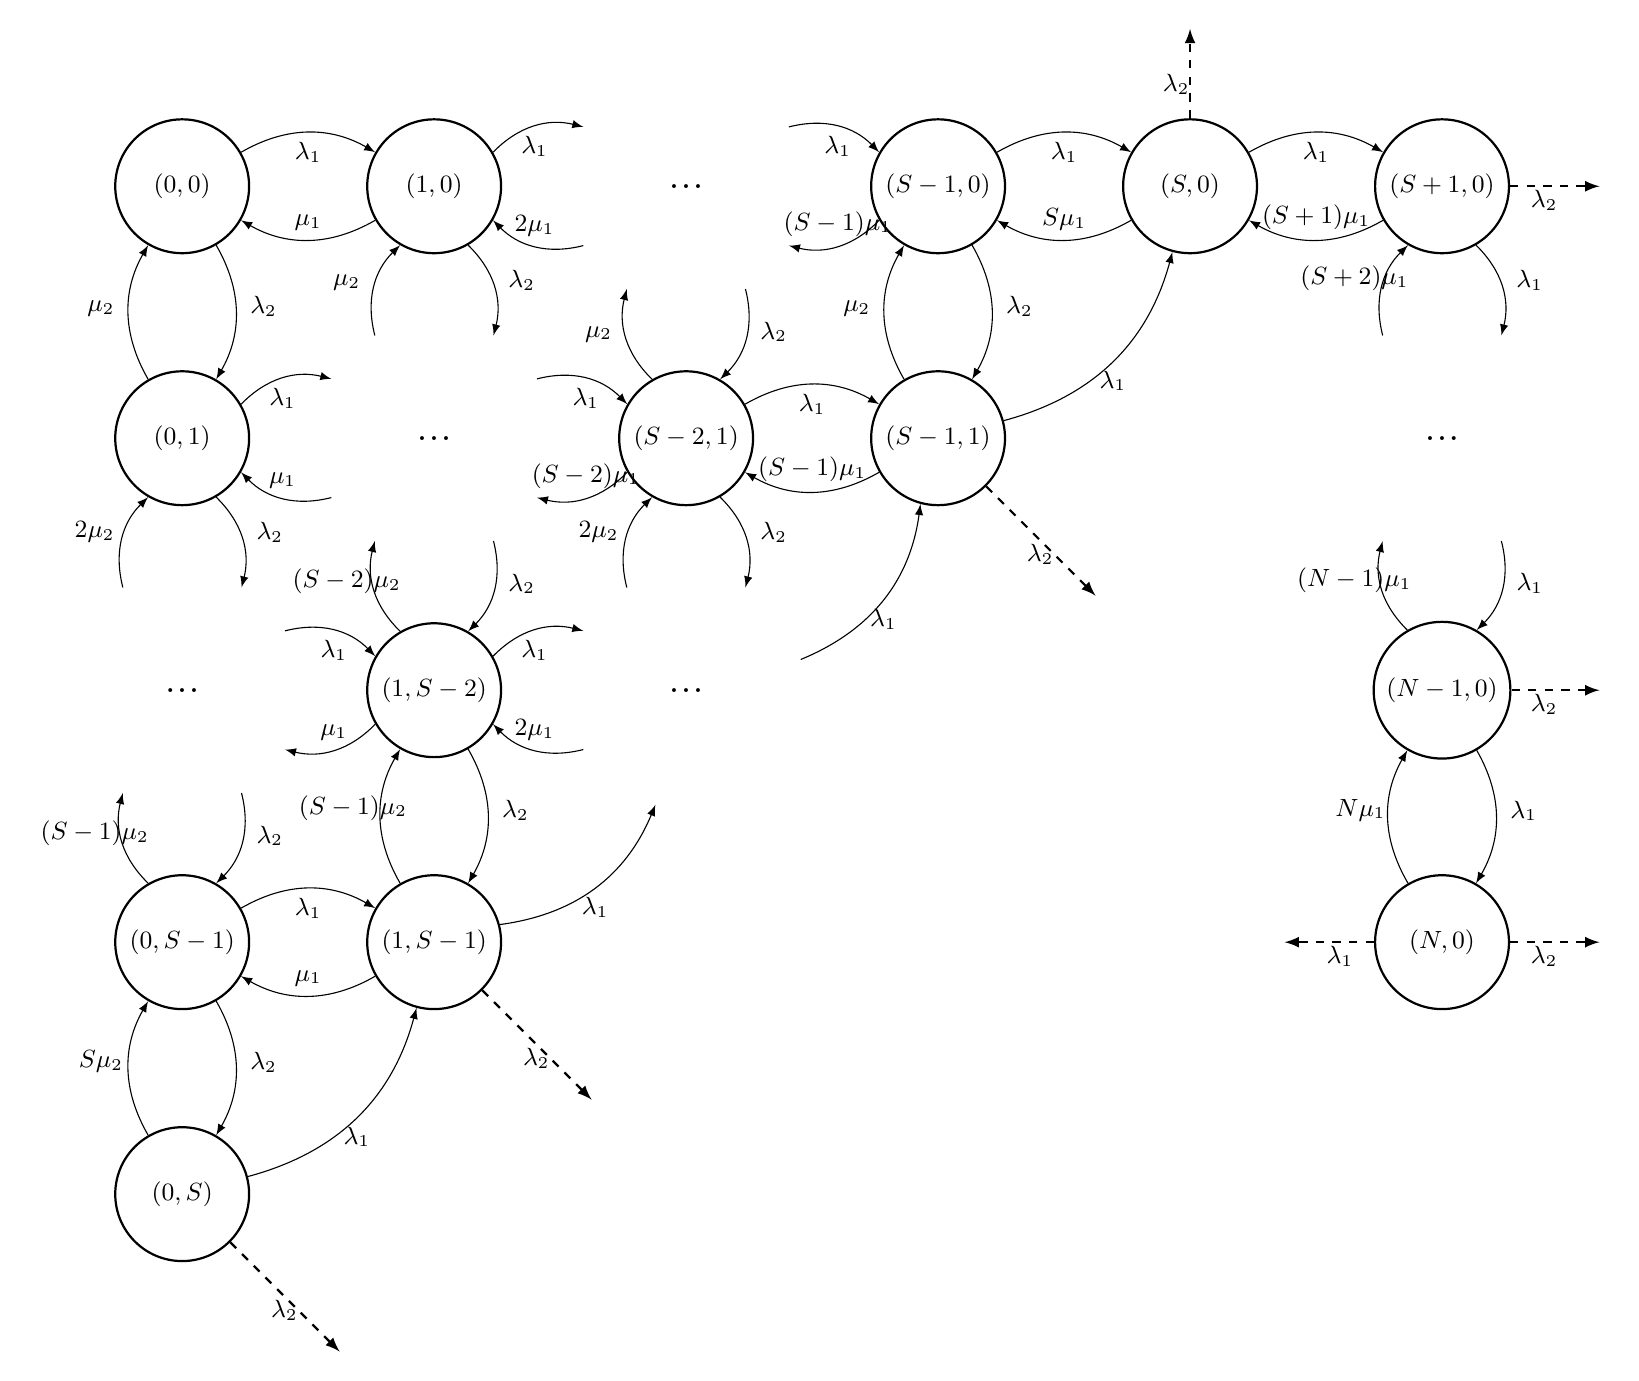
\begin{tikzpicture}[->,node distance=3.2cm,>=latex,font=\small, minimum width=1.7cm]

    \tikzstyle{round}=[thick,draw=black,circle]

    \node[round] 			    (00) {$(0,0)$};
    \node[round,right of=00]    (10) {$(1,0)$};
    \node[round,below of=00]    (01) {$(0,1)$};
    
	\node[circle,draw=white,right of=10, minimum width = 3cm]    (B0) {\LARGE ...};
    \node[circle,draw=white,below of=01, minimum width = 3cm]    (B1) {\LARGE ...};    
    
   	\node[round,right of=B0]    (S-1/0)  	{$(S-1,0)$};
   	\node[round,right of=S-1/0] (S0)	 	{$(S,0)$};
    \node[round,below of=S-1/0] (S-1/1)     {$(S-1,1)$};
    \node[round,left  of=S-1/1] (S-2/1)	{$(S-2,1)$};
   
    \node[round,below of=B1]    (0/S-1)  	{$(0,S-1)$};
   	\node[round,below of=0/S-1] (0S)	 	{$(0,S)$};
    \node[round,right of=0/S-1] (1/S-1)     {$(1,S-1)$};
    \node[round,above of=1/S-1] (1/S-2)     {$(1,S-2)$};
    
    
    \node[circle,below of=10, minimum width = 3cm]    (B2) {\LARGE ...};
    \node[circle,draw=white,right of=1/S-2, minimum width = 3cm]    (B3) {\LARGE ...};
   
    \node[round,right of=S0] (S+1/0)	 	{$(S+1,0)$};  
    \node[circle,draw=white,below of=S+1/0, minimum width = 3cm]    (B4) {\LARGE ...};
    \node[round,below of=B4] (N-1/0)	 	{$(N-1,0)$};  
    \node[round,below of=N-1/0] (N0)	 	{$(N,0)$};  
   
    \draw[dashed,thick, ->] (N0) -- +(2,0) node[xshift=-20,yshift=-5]  {$\lambda_2$};
    \draw[dashed,thick, ->] (N0) -- +(-2,0) node[xshift=20,yshift=-5]  {$\lambda_1$};
    
    \draw[dashed,thick, ->] (N-1/0) -- +(2,0) node[xshift=-20,yshift=-5]  {$\lambda_2$};
    \draw[dashed,thick, ->] (S+1/0) -- +(2,0) node[xshift=-20,yshift=-5]  {$\lambda_2$};
    \draw[dashed,thick, ->] (S0) -- +(0,2) node[xshift=-5,yshift=-20]  {$\lambda_2$};
    \draw[dashed,thick, ->] (1/S-1) -- +(2,-2) node[xshift=-20,yshift=15]  {$\lambda_2$};
    \draw[dashed,thick, ->] (S-1/1) -- +(2,-2) node[xshift=-20,yshift=15]  {$\lambda_2$};
    \draw[dashed,thick, ->] (0S) -- +(2,-2) node[xshift=-20,yshift=15]  {$\lambda_2$};
   
 	\path 
 	
 	(S+1/0)edge[bend left,above]    node {$(S+1)\mu_1$} 		(S0)
 		   edge[bend left,above]       node [xshift=10,yshift=-5]  {$\lambda_1$} 		(B4)
 	
 	(B4)   edge[bend left,above]       node [xshift=-10,yshift=-5] {$(S+2)\mu_1$} 		(S+1/0)
 		   edge[bend left,above]       node [xshift=10,yshift=-5]  {$\lambda_1$} 		(N-1/0)
 		   
 		   
 	(N-1/0)	 edge[bend left,above]       node [xshift=10,yshift=-5]  {$\lambda_1$} 		(N0)
 			 edge[bend left,above]       node [xshift=-10,yshift=-5] {$(N-1)\mu_1$} 	(B4)
 		   
    (N0) edge[bend left,above]       node [xshift=-10,yshift=-5] {$N\mu_1$} 		(N-1/0)
 	
 	(00) 	edge[bend left,below]		node 					    {$\lambda_1$}		(10)
 		 	edge[bend left,above]       node [xshift=10,yshift=-5]  {$\lambda_2$} 		(01)
 	
 	(10) 	edge[bend left,above]       node 						{$\mu_1$} 			(00)
 		 	edge[bend left,below]		node 					    {$\lambda_1$}		(B0)
 		 	edge[bend left,above]       node [xshift=10,yshift=-5]  {$\lambda_2$} 		(B2)
 	
    (01) 	edge[bend left,above]       node [xshift=-10,yshift=-5] {$\mu_2$} 			(00)
   		 	edge[bend left,below]		node 					    {$\lambda_1$}		(B2)
   	     	edge[bend left,above]       node [xshift=10,yshift=-5]  {$\lambda_2$} 		(B1)
   
    (B0) 	edge[bend left,above]       node 						{$2\mu_1$} 			(10)
    		edge[bend left,above]       node [xshift=10,yshift=-5]  {$\lambda_2$} 		(S-2/1)
    		edge[bend left,below]		node 					    {$\lambda_1$}		(S-1/0)
   		    
    (B1) 	edge[bend left,above]       node [xshift=-10,yshift=-5] {$2\mu_2$} 			(01)
   			edge[bend left,above]       node [xshift=10,yshift=-5]  {$\lambda_2$} 		(0/S-1)
   			edge[bend left,below]		node 					    {$\lambda_1$}		(1/S-2)
   			
   
    (B2) 	edge[bend left,above]       node [xshift=-10,yshift=-5] {$\mu_2$} 			(10)
   		 	edge[bend left,above]       node 						{$\mu_1$} 			(01)
   		 	edge[bend left,above]       node [xshift=10,yshift=-5]  {$\lambda_2$} 		(1/S-2)
   		 	edge[bend left,below]		node 					    {$\lambda_1$}		(S-2/1)
   		 	
    (B3)    edge[bend left,above]       node [xshift=-10,yshift=-5] {$2\mu_2$} 			(S-2/1)
   		    edge[bend left,above]       node 						{$2\mu_1$} 			(1/S-2)   	
   		    edge[bend right,below]		node 					    {$\lambda_1$}		(S-1/1)	 	
   		 	
    (S0) 	edge[bend left,above]       node 						{$S\mu_1$} 			(S-1/0)
 			 edge[bend left,below]		node 					    {$\lambda_1$}		(S+1/0)	
 			 
   	(S-1/0) edge[bend left,below]		node 					    {$\lambda_1$}		(S0)
   			edge[bend left,above]       node [xshift=10,yshift=-5]  {$\lambda_2$} 		(S-1/1)
   			edge[bend left,above]       node 						{$(S-1)\mu_1$} 		(B0)
   
    (S-1/1) edge[bend left,above]       node [xshift=-10,yshift=-5] {$\mu_2$} 			(S-1/0)
    		edge[bend left,above]       node 						{$(S-1)\mu_1$} 		(S-2/1)
    		edge[bend right,below]		node 					    {$\lambda_1$}		(S0)	 
    
    (S-2/1) edge[bend left,below]		node 					    {$\lambda_1$}		(S-1/1)
    		edge[bend left,above]       node [xshift=-10,yshift=-5] {$\mu_2$} 			(B0)
    		edge[bend left,above]       node 						{$(S-2)\mu_1$} 		(B2)
    		edge[bend left,above]       node [xshift=10,yshift=-5]  {$\lambda_2$} 		(B3)
		 
    (0S) 	edge[bend left,above]       node [xshift=-10,yshift=-5]	{$S\mu_2$} 			(0/S-1)
    		edge[bend right,below]		node 					    {$\lambda_1$}		(1/S-1)
   
   	(0/S-1) edge[bend left,below]		node 					    {$\lambda_1$}		(1/S-1)
   			edge[bend left,above]       node [xshift=10,yshift=-5]  {$\lambda_2$} 		(0S)
   			edge[bend left,above]       node [xshift=-10,yshift=-5]	{$(S-1)\mu_2$} 		(B1)
   
    (1/S-1) edge[bend left,above]       node 						{$\mu_1$}  			(0/S-1)
    	    edge[bend left,above]       node [xshift=-10,yshift=-5]	{$(S-1)\mu_2$} 		(1/S-2)
    	    edge[bend right,below]		node 					    {$\lambda_1$}		(B3)
    
    (1/S-2) edge[bend left,above]       node 						{$\mu_1$}  			(B1)
    		edge[bend left,above]       node [xshift=10,yshift=-5]  {$\lambda_2$} 		(1/S-1)
    		edge[bend left,above]       node [xshift=-10,yshift=-5]	{$(S-2)\mu_2$} 		(B2)
    		edge[bend left,below]		node 					    {$\lambda_1$}		(B3)
  
    		
   ;
  
\end{tikzpicture}
\end{adjustbox}
\end{figure}

\begin{adjustbox}{center=\textwidth}
\label{equation:AccessControlAlgorithm1-BalanceEquations}

$\begin{cases} 
(\lambda_1 + \lambda_2)\pi_{(0,0)} = \mu_1\pi_{(1,0)} + \mu_2\pi_{(0,1)} \\

(\lambda_1 + \lambda_2 + i\mu_1)\pi_{(i,0)} = \lambda_1\pi_{(i-1,0)} + \mu_1(i+1)\pi_{(i+1,0)} + \mu_2\pi_{(i,1)} & \forall i \in \mathbb{N} \mid 1 \leq i \leq S-1 \\

(\lambda_1 + \lambda_2 + i\mu_2)\pi_{(0,i)} = \lambda_2\pi_{(0,i-1)} + \mu_1\pi_{(1,i)} + \mu_2(i+1)\pi_{(0,i+1)} & \forall i \in \mathbb{N} \mid 1 \leq i \leq S-1 \\

(S\mu_1+\lambda_1)\pi_{(S,0)} = \lambda_1\pi_{(S-1,0)} + \lambda_1\pi_{(S-1,1)} + (S+1)\mu_1 \pi_{(S+1,0)}\\

(\lambda_1 + S\mu_2) \pi_{(0,S)} = \lambda_2\pi_{(0,S-1)} \\

(i\mu_1 + j\mu_2 + \lambda_1)\pi_{(i,j)} = \lambda_1\pi_{(i-1,j)} + \lambda_2\pi_{(i,j-1)} & \forall i,j \in \mathbb{N} \mid \begin{array} {l} 1 \leq i \leq S-1 \\ 1 \leq j \leq S-1 \end{array} \mid i + j = S \\

(\lambda_1 + \lambda_2 + i\mu_1 + j\mu_2)\pi_{(i,j)} = \lambda_1\pi_{(i-1,j)} + \lambda_2\pi_{(i,j-1)} + \mu_1(i+1)\pi_{(i+1,j)} + \mu_2(j+1)\pi_{(i,j+1)} & \forall i,j \in \mathbb{N} \mid \begin{array} {l} 1 \leq i \leq S-1 \\ 1 \leq j \leq S-1 \end{array} \mid i + j < S \\

(i\mu_1 + \lambda_1)\pi_{(i,0)} = \mu_1(i+1)\pi_{(i+1,0)} + \lambda_1\pi_{(i-1,0)} & \forall i \in \mathbb{N} \mid S+1 \leq i \leq N-1 \\

N\mu_1\pi_{(N,0)} = \lambda_1\pi_{(N-1,0)} \\

\sum \pi_{(i,j)} = 1 & \forall i,j \in \mathbb{N}_0

\end{cases}
$ 
\end{adjustbox}

\subsubsection{Probabilities computing}

although... To properly analyse this system, we need do compute some useful probabilities.

Similarly to the previous case we need to now following probabilities:



\begin{table}[h!]
    \caption{Lista dei file del malware FASTCash}
    \centering
    \small
    \label{tab:MalwareFileList}
     \begin{tabular}{rp{8cm}}

      \toprule

      $\Pi_{\text{SendToCloudlet}}(k)$ & Probability that an arriving job of class $k$ on controller has to be forwarded to cloudlet \\
\\
      $\Pi_{\text{SendToCloud}}(k)$ & Probability that an arriving job of class $k$ on controller has to be forwarded to cloud \\
\\
      $\Pi_{\text{Class2JobInterruption}}(k)$ & Probability that a job of class 2 running on cloudlet has to be interrupted and forwarded to cloud due of  arriving class 1 job on cloudlet. \\

      \bottomrule

    \end{tabular}
\end{table}

Differently from the previous case, owing to the use of a different access control algorithm, jobs of different classes have different probability according to which an arriving job on controller has to be send to cloud. From CTMC analysis, we can easily understand that:


\begin{equation}
\begin{array} {lcl} 
\Pi_{\text{SendToCloud}}(1) & = & P\lbrace{\text{An arrival class 1 job on controller sees $N$ class 1 jobs in cloudlet}}\rbrace \\ 
\\
& = & P\lbrace{n_1 = N}\rbrace \\ 
\\
& = & \pi(N,0)
\end{array}
\end{equation}



\begin{center}
\begin{equation}
\begin{array} {lcl} 
\Pi_{\text{SendToCloud}}(2) & = & P\lbrace{\text{An arrival class 2 job on controller sees that number of jobs in cloudlet exceed or is equal to a given threshold S}}\rbrace \\ 
\\
& = & P\lbrace{n_1 + n_2 \geq N}\rbrace \\ 
\\
& = & \displaystyle \sum_{\substack{n_1,n_2 = 0 \\ n_1 + n_2 = S}}^{S} \pi(n_1,n_2) + \sum_{n_1 = S+1}^{N}\pi(n_1,0) \\
\\
& = & \displaystyle \sum_{\substack{0 \leq n_1 \leq N \\ 0 \leq n_2 \leq S \\ n_1 + n_2 \geq S}} \pi(n_1,n_2)
\end{array}
\end{equation}
\end{center}

\end{document}
